\chapter{Introduction}
Imagine we play the Catch Phrase game, in which you are
first presented a word and then try to get me to guess this
word by describing the object without saying a word that rhymes with the given word, or giving the first letter of the word, or saying the number of syllables or part of the word.
Further imagine you were given the word \emph{cell}, how 
would you describe it? If you come up with \emph{round,
liquid, life, etc.}, I might probably have guessed 
\emph{apple}. On the other hand, it is highly unlikely that 
you will say such keywords as
\emph{dynamic, network, complex system, etc.}, since one 
usually assumes all these relate to certain man-made 
objects, e.g. airplane or even Facebook. 
But if you combine these two sets of clues, I think
the answer will be unique, namely \emph{cell} without doubt.

%Transcriptome is the total set of transcripts, or mRNA and other non-coding RNAs
%within the cell. Unlike the genome, which acts as a template for different life
%forms, transcriptome can vary according to the context, i.e. specific tissues or
%external stimuli. In addition, the dynamics of gene expression roughly coincides 
%with that of the cellular phenotype, which makes the study of transcriptome 
%especially promising. 
In this chapter, we would like to motivate the reason 
why keywords such
as \emph{dynamic, network, complex system} can be linked
to the cell.
We first summarize the current knowledge about
the cellular response to stimulus from a biological point of
view, and then highlight the need to approach the problem
within the theoretical context of complex systems. 
Both the dynamic and 
network aspect of cellular networks will be presented. 
Finally, we also lay out the roadmap for the following 
chapters.

\section{Cellular signal processing}
Cells are the building blocks of all living organisms except viruses. As an 
independent functional unit, individual cells sense the environmental cues 
(such as cytokine or growth factor stimulation, extracellular matrix interactions, DNA damage, or osmotic stress) by the membrane receptors. The latter
then activate a cascade of protein reaction and modification in the cytoplasm,
which leads to the gene regulation being triggered by 
DNA-binding proteins, i.e. transcription factors. Post-transcriptional
regulations again forms feedback loops at various levels, which act upon the
upstream signaling proteins (\ref{fig:signal_flow}).

\begin{figure}[!ht]
\begin{center}
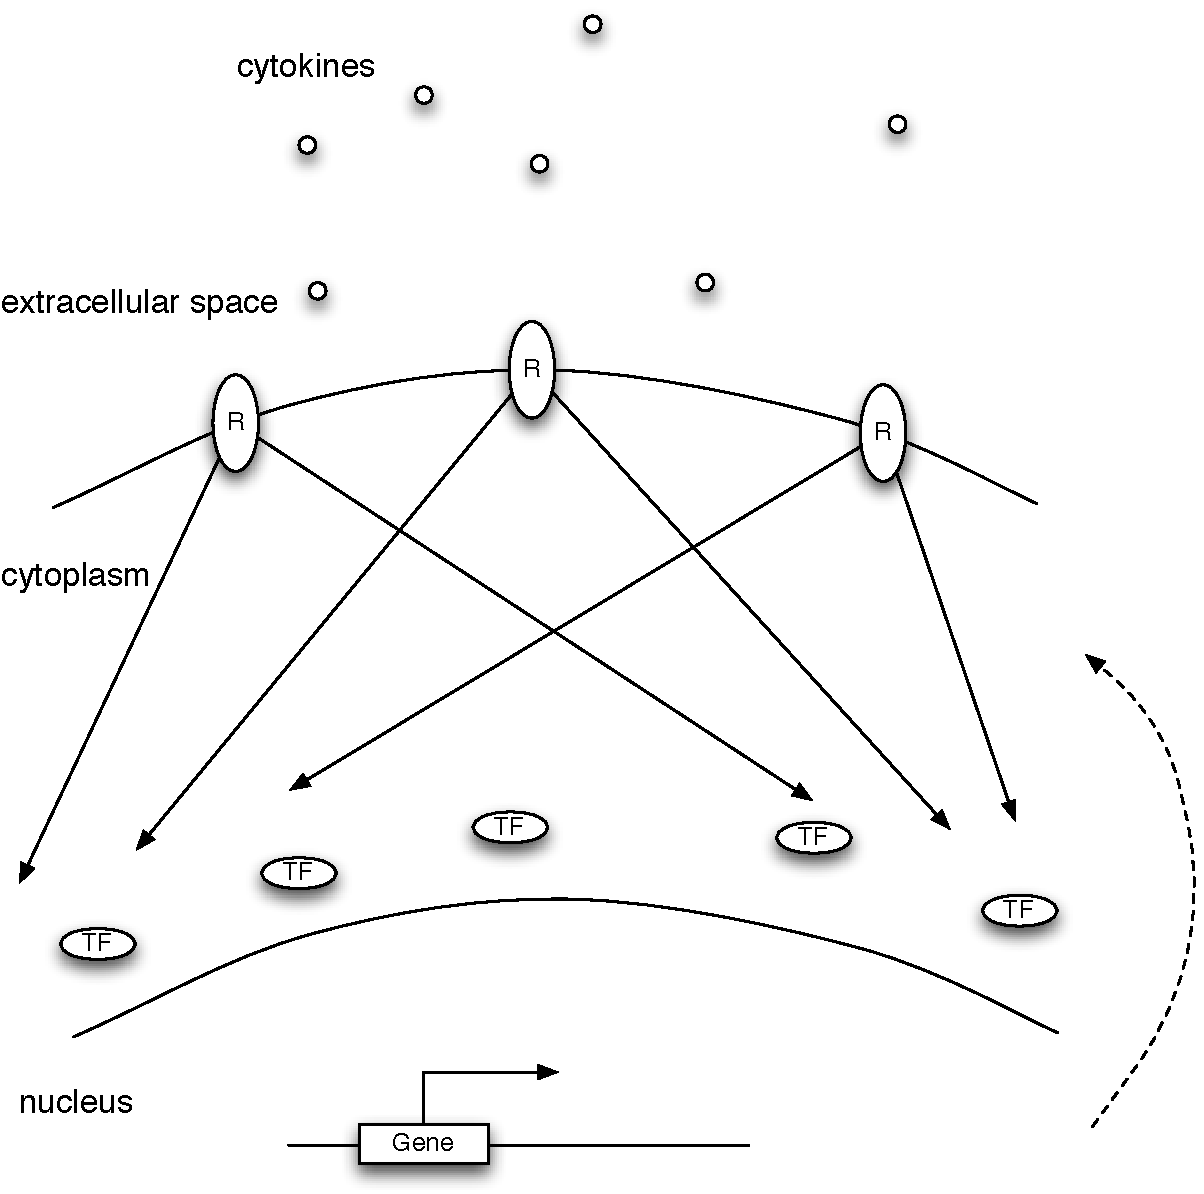
\includegraphics[width=0.8\textwidth]{signal_flow.pdf}
\end{center}
\caption[Signal flow]{{\bf Schematic view of signal flow from membrane 
receptors to gene regulation in the eukaryotic cell.}
Signal flow in the interactome and the transcriptional 
regulatory network are two temporally separated processes 
with
fast and slow dynamics respectively. In eukaryotic cells,
these two processes are also spatially separated by the
nucleus.
}
\label{fig:signal_flow}
\end{figure}

How cells transmit signal\footnote{In the following we
use \emph{signal} and \emph{information} interchangably.} 
has long been an active research topic.
The last decades have witnessed the transition from a classical view of 
simple linear signaling pathways
to the idea of an intertwingled signaling network coordinating multiple 
pathways~\citep{Kholodenko2012}. Techniques as yeast two hybrid system 
and mass spectrometry based
proteomics have greatly enhanced the ability to map the components of such 
signal transduction networks. Despite the inherent large number of false
positive hits from such high-throughput studies~\citep{Mering2002a}, 
efforts have been devoted
to collect different sources of protein-protein interaction 
(PPI) data, such as BioGRID%
~\citep{Stark2006} and STRING~\citep{Szklarczyk2011}. Recently, the HIPPIE
database~\citep{Schaefer2012} was proposed to integrate multiple experimental PPI
data sources and assign a score to each interaction. This
score is normalized by the number of publications reporting 
a certain
interaction, the quality of the experimental technique used
to detect this interaction, and how conserved this particular
interaction is across species. Such efforts have greatly 
contributed to the current knowledge of protein interactions
and therefore the backbone of the signal propagation network.

Proteins interact with and modify each other most often by phosphorylation.
By further investigating the time-resolved phosphorylation
events, one gets additional information about some general
and context-specific mechanisms of the signal flow.
For instance, in a phospho-proteomic study of 
HeLa cells stimulated with epidermal growth factor (EGF)~%
\citep{Olsen2006},
it was found that the majority of proteins contain multiple 
phosphorylation sites showing different kinetics, which 
suggests that they serve as platforms for integrating 
signals. As another example, a phospho-proteomic analysis
of the human embryonic stem cell differentiation in response
to different stimuli~\citep{Rigbolt2011} reveals interesting
dynamic phosphorylation of DNA methyltransferases, which
regulate several pluripotency marker genes and thereby 
providing a link between the differential signal and the
downstream transcriptional machinery.

After reaching the transcription factor, 
the cellular signal switches from the
protein activity to the transcription of the target genes. The transcription,
or copy of a certain gene is strictly controlled by the transcription factor,
which binds to the promoter region of the gene and initiates the production
of a messenger RNA. The messenger RNA is then translated into proteins,
which join the signal processing cascade and can change certain cellular 
phenotypes. Thus the information flow from membrane receptors to transcription
factors, which induce the gene expression and subsequently protein synthesis, 
forms a feedback regulatory loop.

\section{Predictive analysis and systems biology}
Four great ideas, as Sir Paul Nurse once argued~%
\citep{Nurse2003}, are core to biology. These are what
modern biologists take for granted now: (i) the gene is the basis for heredity, (ii) the cell is the fundamental unit of organisms, (iii) biology is based on chemistry, and (iv) species evolve by natural selection. And a possible fifth great 
idea is the emerging view that biological organisation is explained in terms of logical
and informational processes and structures. 
In other words, 
the new fundamental idea presupposes that biology is only to be 
understood
on the level of complex systems formed by interacting genes and macromolecules, or cells at a higher scale~%
\citep{Vidal2009}.

The accumulation of various proteomic and transcriptomic
data poses both an opportunity and a challenge of 
generating a coherent 
mechanistic picture of cellular decision-making on the 
system level. In many
other different fields, data-driven predictions have 
emerged to be the \emph{de facto} everyday routine. Weather
forecasting services use information like temperature, 
precipitation, wind speed to predict the state of the 
atmosphere at a given location in the near future. Google
Flu Trends is an integrative platform to detect influenza
epidemics based on health-seeking behaviour in the form of 
web queries~\citep{Ginsberg2009}. In the 2012 US presidential
election, the team of Barack Obama had made better use of 
voters' TV viewing habits and certain personal information 
to identify likely supporters and
approach them most efficiently with direct advertising. 
This strategy helped Obama to beat the better-financed
Republican opponent.

Predictive modeling of biological data ranges from the 
abstract 
data-driven modeling framework (including clustering and 
regression methods) to the mechanistic differential 
equation-based modeling, with Bayesian networks, Boolean
logic and other methods lying in between~\citep{deJong2002}. 
While the lab work remains time- and labor-intensive, 
theoretical 
modeling approaches have helped to gain insights into how
the signal processing unit in the cell works.
For example, it is observed that only
weak, sustained EGF receptor (EGFR) phosphorylation can be
translated into the phosphorylation of ribosomal protein 
S6, a molecule downstream in the Akt pathway of PC12 cells~%
\citep{Fujita2010}. Frequency domain analysis reveals that 
the Akt pathway exhibits the property of a low-pass filter,
namely only transmitting low-frequency signals to the 
downstream effectors. This led to the somewhat 
counter-intuitive hypothesis that in a pathway with low-pass filter properties, any upstream inhibitor that can convert a strong transient time course into a weak sustained time course can be a potential downstream activator, which might 
explain certain aspects of drug resistance or side-effects
in different EGFR inhibitor treatments~\citep{Kosaka2011,
Lin2012}.

Unlike the weather and flu forecasts, however, predictive
analysis is not the aim, but rather a means to study 
biological systems. Instead of a one-way street that leads
from data to model and finally predictions, systems biology
is rather a cycle (\ref{fig:sb_cycle}) 
that starts from describing the current
biological knowledge by a mathematical model, simulation of
the model then generates multiple testable hypotheses, which
are in turn validated in wet experiments~%
\citep{Kitano2002e}. An analogy can be drawn between the
cycle of systems biology and the working principles in many
engineering disciplines. In order to build airplanes, 
automobiles, or bridges, buildings, it is usually required
to first construct a physical \emph{model} of the object
and study the airflow around that object in a wind tunnel.
The measurements from this \emph{experiment} can then be 
used to improve the design of such objects in an iterative
fashion.

\begin{figure}[!ht]
\begin{center}
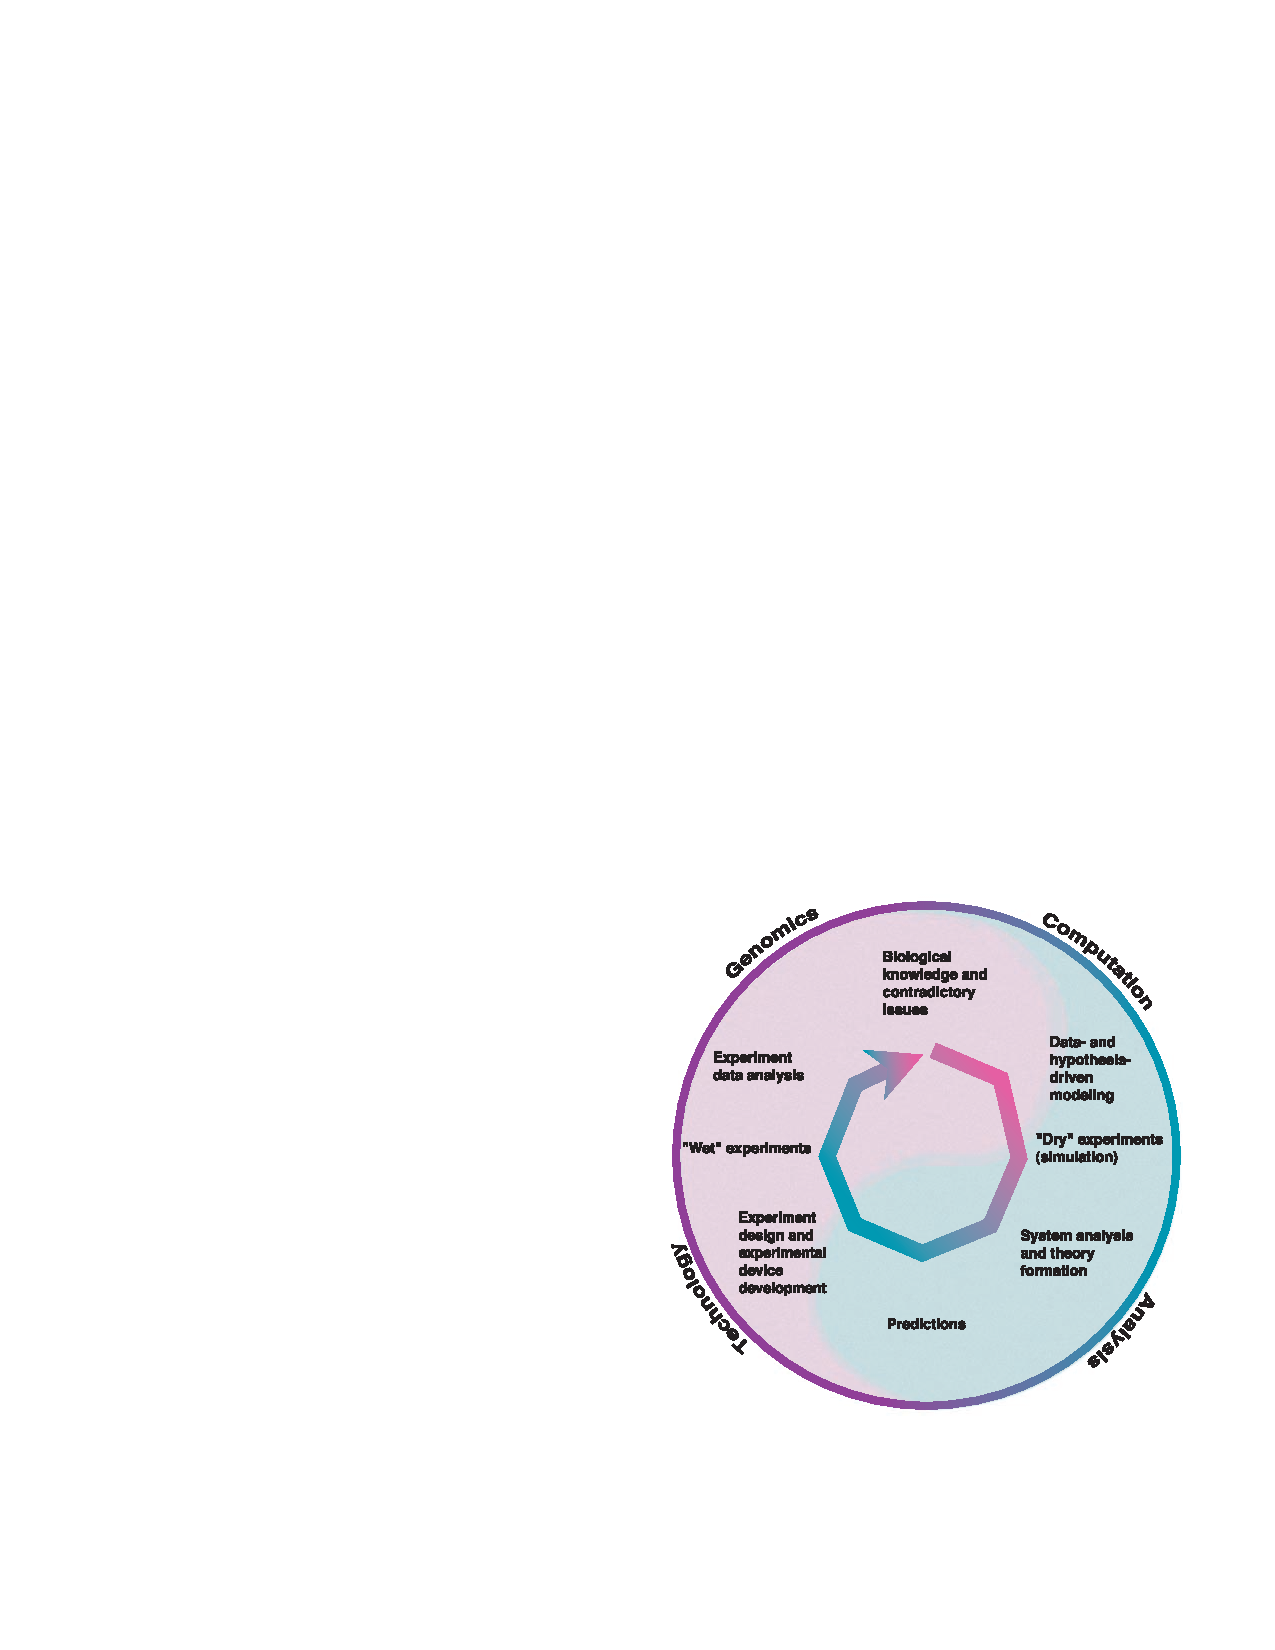
\includegraphics[width=0.8\textwidth]{sb_cycle.pdf}
\end{center}
\caption[Cycle of systems biology]{{\bf The systems biology
research can be represented by a cycle that iterates between
models and experiments.} 
Taken from \cite{Kitano2002e}.
}
\label{fig:sb_cycle}
\end{figure}

\section{Complex dynamical system}
A complex system is a system with a large number of
elements, building blocks or agents, capable of interacting
with each other and with their environment.
The
active field of systems biology provides exactly a formal,
quantitative language to describe complex biological 
systems, and
bridges the gap between biology and other well-established
mathematical and engineering disciplines. 

It is widely believed that beginning with the general 
systems theory formulated some 
60 years ago by Ludwig von Bertalanffy, cells have been
approached as complex systems~\citep{Lazebnik2002a}. 
However, the root of systems approaches in biology and
medicine probably can be traced back as far as two 
thousand years
ago, when the traditional Chinese medicine (TCM) was 
founded. TCM obtains information from patients by 
inspection, 
listening and smelling, inquiry, and pulse-taking. 
It considers the various parts of the 
human body as an organic whole and as part of the 
universe, and the various organs closely 
related to each other physiologically and pathologically. 
The treatment is based on the 
differentiation of syndromes and a typical prescription
consists of multiple herbs with about 9 to 18 substances.
This is in stark contrast to the common single drug
target strategy in most \emph{western} medicine.

Therefore, systems biology can heavily profit from the
study of complex systems.
Advanced technologies and biology have different physical
implementations, yet similar systems-level organization
principles. Both domains produce modular architectures that are composed of elaborate hierarchies and feedback regulation, both are featured by demand for
robustness to uncertain environments~\citep{Csete2002}.
The
finding, in physical systems, of universal properties that
are independent of the specific form of the interactions
gives rise to the intriguing hypothesis that universal laws
or results may also be present in complex social, economic
and biological systems~\citep{Amaral2004}. One example is 
the recent finding that the melting dynamics of glaciers
resembles the firing events of spiking neurons~%
\citep{Chapuis2012}.

Although we are now able to describe some of the individual 
components of the 
signalling network in detail, we still do not understand how they operate together to generate biological specificity. It is like trying to plan a journey with an incomplete railway network map lacking train time schedules. Even the simple transport of a signal requires both a network map and a time schedule,
because all trains use common tracks, but shifting their 
running time can determine which connections are enabled or disabled~\citep{Kholodenko2010}.
Therefore, the study of emergent properties of signalling networks encoded by temporal dynamics becomes more and more
appreciated.

Probably one of the most prominent examples linking network
dynamics and phenotypic response comes from observations 
that the duration of extracellular signal-regulated kinase (ERK) activation correlates with cell fate decisions in rat pheochromocytoma PC12 cells. More specifically, transient ERK activation by epidermal growth factor (EGF) induced cell proliferation, whereas sustained ERK activation by nerve growth factor (NGF) induced differentiation~\citep{Marshall1995a}.

Likewise, although missing a direct functional mechanism, the link between the molecular 
dynamics of certain proteins/genes and the cellular phenotype has been observed in the yeast.
In yeast, secreted pheromones activate MAPK signalling in cells of the opposite mating type, resulting in the formation of mating projections. A recent study shows that in these cells, oscillations of Fus3 MAPK activity are observed on the same timescale (2--3 hours) as the periodic formation of additional mating projections~\citep{Hilioti2008}. 

\section{Network}
The difficulty of identifying biomarker molecules to diagnose diseases, stratify patients, and predict responses to therapies is
largely recognized. However, it is still a striking figure
that less than 1\% of all published cancer biomarkers ever 
enter clinical practice~\citep{Kern2012}. Among the various
reasons of failure, it is the function and malfunction of signaling networks that are often closely linked to pathogenic mechanisms. Hence, cellular networks, instead of single
molecules, may prove to be better suited as biomarkers~%
\citep{Barabasi2011,Chuang2007,Chu2008}.
Similarly, consciousness cannot be reduced to or explained by any single 
neuron. It is rather an emergent property that engages 
the interaction between billions of them. 

Because networks are so ubiquitous
in science as well as our daily life, it is beneficial to
study the abstract representation of different complex 
systems as networks. Network theory aims to understand the origins and characteristics of networks that hold together the components in various complex systems. The more we look
into networks of different nature, the more we come to 
realize that networks behind most complex systems are governed by a series of fundamental laws that determine and limit their behaviour. 
It is therefore believed that in general complexity can only be understood within the
network context~\citep{Barabasi2012}. 
Network theory is also fundamentally different
from any other theory in the way that 
it heavily relies on and is inspired by
empirical real-world data, which are again only made 
available recently with the advance of various technologies.
 
%Furthermore, it is not sufficient to know all the components
%within the network. What is much more crucial is the 
%knowledge about the wiring diagram of the network,
%and understanding a complex network's 
%structure is beneficial to understanding its function.

A variety of biological networks including protein-protein interaction, protein-DNA interaction, and RNA interaction networks are essential to cooperative biological activities~\citep{Zhu2007a}. These networks consist of nodes (vertices) which denote molecules, and links (edges) which denote interactions between them. Depending on the type of interaction, the corresponding edge might be directed or undirected. For example, a binding between two proteins is usually represented as an undirected edge while an interaction between a transcription factor and a gene whose expression is regulated by the given transcription factor is usually represented as a directed edge where the direction goes from the transcription factor to the gene.

If the cellular phenotype is indeed encoded in interaction 
networks, one would expect that the development of 
phenotype can be predicted by studying the cellular
networks. By integrating a coexpression network, seeded with four well-known breast cancer
associated genes, together with genetic and physical interactions, \cite{Pujana2007} yielded a breast cancer network model, out of which candidate cancer susceptibility and modifier genes could be predicted.
\cite{Zhong2009} studied the
perturbations of cellular networks, which can result in phenotypic variations.
The type of the perturbation ranges from node removal at one end and edge-specific,
\emph{edgetic} perturbations at the other. The
consequences on network structure and function are shown
to be radically dissimilar for node removal versus edgetic perturbation. Node removal not only disables the function of a node but
also disables all the interactions of that node with other nodes,
disrupting in some way the function of all of the neighboring nodes. An edgetic disruption, in contrast, removes one or a few interactions
but leaves the rest intact and functioning, and has thus 
subtler effects
on the network. 

\section{Outline of the thesis}
In this thesis, we intend to provide a global network
perspective on how cells make decisions as to proliferation,
apoptosis, differentiation or migration.

We begin \ref{chap:network} by introducing several 
topological and dynamical measures to characterize gene
regulatory networks. By synthesizing \emph{in silico}
networks and simulating their dynamics using a 
thermodynamical model,
we further determine the relative
contribution of topological and dynamical factors to the 
general response of the network. Topology is found to have
a greater impact on network response in both \emph{in silico}
and biological networks. Furthermore, we found that strongly
regulated and sparsely connected genes correlate with the
cellular phenotype, which is also confirmed by a series
of inhibition experiments in an \emph{in vitro} mammalian
system.

In \ref{chap:flow}, we continue with the question in mind:
what caused the transcriptome response that ultimately leads
up to the cellular fate decision and change of phenotype?
Before exploring the signalling pathways linking membrane
receptors and transcriptional regulators, we review several
widespread enrichment analyses to identify activated or
deregulated pathways from the transcriptome data. We then
propose a two-step integrative approach that separates two distinct 
time scales of protein and gene regulation. 
Signal flow in the interactome is represented by the 
proximity between membrane receptors and transcription 
factors. We further compare two such distance metrics, i.e.
shortest path length and mean first passage time. The
usefulness of the latter metric is demonstrated in a study of
tumor-stroma interaction.

The thesis is finally concluded with a discussion of some
of the intriguing implications from our results.
